The planning module is divided in three different parts.

\begin{enumerate}
    \item The first thing to do is to find a goal point, that goal point must be chosen in a way that will make the robot explore unknown parts of the environment.
    \item Then we have to build a path for the robot to follow between the actual position of the robot and the target.
    \item The final thing to do is to use a path tracking algorithm that will make the robot follow the built path.
\end{enumerate}

\section{Find a goal point}

In order to find a goal point we have to detect an unexplored zone that we can access to, to do so we used an approach based on frontier detection.
A frontier is a region on the border between an explored zone and an unexplored zone.
Then the first thing to do in order to determine the next goal point is to detect the frontiers.

\subsection{Detect the frontiers}

At first we thought that a naive approach could be enough for this part, but we later noticed that it was not efficient enough.

\subsubsection{First naive approach}

To detect the frontiers we go through all the unexplored cells of the grid and if that cell has an explored empty cell in its Von Neumann neighbourhood we know it is part of a frontier.
The Von Neumann neighbourhood is composed of the four adjacent cells around a cell.
Once we went through the whole grid we have a list of all the cells that are on a frontier, the next step is to divide them into several regions.

To divide the frontiers in regions we go through the previously built list, each time we put a cell in its region we delete it from the initial list.
For each cell we go through its Moore neighbourhood (The entire 8 cells neighbourhood).
If one of its neighbour is in the initial list we recursively call the same function.

This is the pseudocode of the 'get\_divided\_frontiers' function:

\FloatBarrier
\begin{algorithm}
    \caption{get divided frontiers}
    \label{get divided frontiers}
    \begin{algorithmic}[1]
        \Procedure{get\_frontiers}{$map$}
            \State $frontiers$ is an empty array
            \For{$cell$ \textbf{in} $map$}
                \If{$is\_unknown(cell)$}
                    \For{$neighbour$ \textbf{in} $von\_neumann\_neighbourhood(cell)$}
                        \If{$neighbour$ \textbf{not in} $frontiers$ \textbf{and} $is\_empty(neighbour)$}
                            \State $frontiers.append(neighbour)$
                        \EndIf
                    \EndFor
                \EndIf
            \EndFor
            \State \textbf{return} $frontiers$
        \EndProcedure
        \Procedure{build\_frontiers}{$frontiers,$ $current\_frontier,$ $cell$}
            \State $neighbours \gets moore\_neighbourhood(cell)$
            \For{$neighbour$ \textbf{in} $neighbours$}
                \If{$neighbour$ \textbf{in} $frontiers$}
                    \State $current\_frontier.append(neighbour)$
                    \State $frontiers.remove(neighbour)$
                    \State $build\_frontier(frontiers, current\_frontier, cell)$
                \EndIf
            \EndFor
        \EndProcedure
        \Procedure{get\_divided\_frontiers}{$map$}
            \State $frontiers \gets get\_frontiers$
            \State $divided\_frontiers$ $is$ $an$ $empty$ $array$
            \While{$frontiers$ \textbf{is not} $empty$}
                \State $current\_frontier$ $is$ $an$ $empty$ $array$
                \State $cell \gets frontiers.pop(0)$
                \State $current\_frontier.append(cell)$
                \State $build\_frontier(frontiers, current\_frontier, cell)$
                \State $divided\_frontiers.append(current\_frontier)$
            \EndWhile
            \State \textbf{return} $divided\_frontiers$
        \EndProcedure
    \end{algorithmic}
\end{algorithm}
\FloatBarrier

On the following figure we can see an example of the detected frontiers, the black pixels are obstacles, the white ones are empty cells, the red spot is the robot position and the other spots are the regions of frontiers. 
The map is 10 by 10 and there is a different color for each region.
By testing this same function on a real map built by the robot in MRDS we noticed that despite being theoretically precise it is not efficient enough (it took around 5 to 10 seconds to get the frontiers).
However, the function gave a very good result as we can see below:

\begin{figure}[h]
    \centering
    \begin{subfigure}{.5\textwidth}
        \centering
        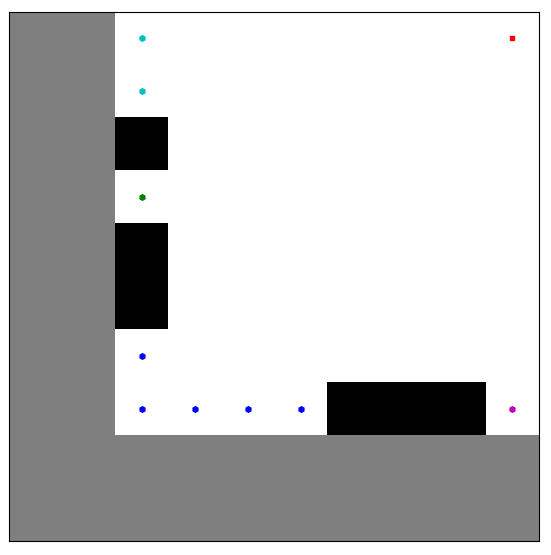
\includegraphics[height=\linewidth]{frontiers.png}
        \caption{Frontiers test map}
        \label{fig:frontiers}
    \end{subfigure}%
    \begin{subfigure}{.5\textwidth}
        \centering
        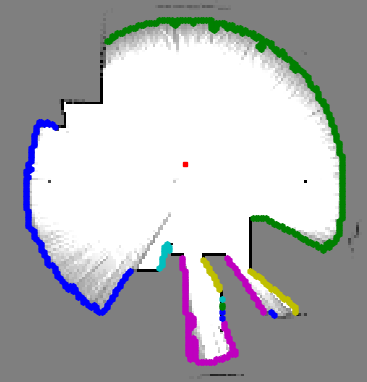
\includegraphics[height=\linewidth]{frontiers_real_map.png}
        \caption{Frontiers real map}
        \label{fig:frontiers_real_map}
    \end{subfigure}
\end{figure}

\subsubsection{Final approach, the Wavefront Frontier Detector algorithm}

We found this algorithm in a scientific paper, happily there was a very comprehensible pseudocode in the paper that we simply followed to implement it in our project.

This is the pseudocode of the algorithm:

\FloatBarrier
\begin{algorithm}
    \caption{Wavefront Frontier Detector}
    \label{wavefront_frontier_detector}
    \begin{algorithmic}[1]
        \State $queue\_m \gets []$
        \State $queue\_m.append(robot\_cell)$
        \State $frontiers \gets []$
        \State $map\_open \gets set([])$
        \State $map\_close \gets set([])$
        \State $frontier\_open \gets set([])$
        \State $frontier\_close \gets set([])$
        \State $map\_open.add(robot\_cell)$
        \While{$queue\_m$ \textbf{is not empty}}
            \State $p \gets queue\_m.pop(0)$
            \If{$p$ \textbf{in} $map\_close$}
                \State \textbf{continue}
            \EndIf
            \If{$is\_frontier\_point(p)$}
                \State $queue\_f = []$
                \State $frontier \gets set([])$
                \State $queue\_f.append(p)$
                \State $frontier\_open.add(p)$
                \While{$queue\_f$ \textbf{is not empty}}
                    \State $q \gets queue\_f.pop(0)$
                    \If{$q$ \textbf{in} $map\_close$ \textbf{and} $q$ \textbf{in} $frontier\_close$}
                        \State \textbf{continue}
                    \EndIf
                    \If{$is\_frontier\_point(q)$}
                        \State $frontier.add(q)$
                        \For{$w$ \textbf{in} $moore\_neighbourhood(q)$}
                            \If{$w$ \textbf{not in} $frontier\_open$ \textbf{and} $w$ \textbf{not in} $map\_close$ \textbf{and} $w$ \textbf{not in} $frontier\_close$}
                                \State $queue\_f.append(w)$
                                \State $frontier\_open.add(w)$
                            \EndIf
                        \EndFor
                    \EndIf
                    \State $frontier\_close.add(q)$
                \EndWhile
                \State $frontiers.append(frontier)$
                \For{$cell$ \textbf{in} $frontier$}
                    \State $map\_close.add(cell)$
                \EndFor
            \EndIf
            \For{$v$ \textbf{in} $moore\_neighbourhood(p)$}
                \If{$v$ \textbf{not in} $map\_open$ \textbf{and} $v$ \textbf{not in} $map\_close$ \textbf{and} $has\_open\_neighbour(v)$}
                    \State $queue\_m.append(v)$
                    \State $map\_open.add(v)$
                \EndIf
            \EndFor
            \State $map\_close.add(p)$
        \EndWhile
        \State \textbf{return} $frontiers$
    \end{algorithmic}
\end{algorithm}
\FloatBarrier

Those are the frontiers detected with this new algorithm in a test and a real case, in the real case we only displayed the frontiers with more than 20 points in it.

\begin{figure}[h]
    \centering
    \begin{subfigure}{.5\textwidth}
        \centering
        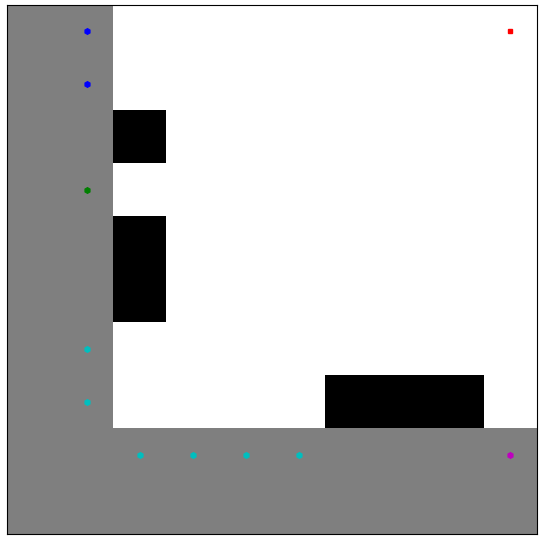
\includegraphics[width=\linewidth]{frontiers_wfd.png}
        \caption{Frontiers test map WFD}
        \label{fig:frontiers_wfd}
    \end{subfigure}%
    \begin{subfigure}{.5\textwidth}
        \centering
        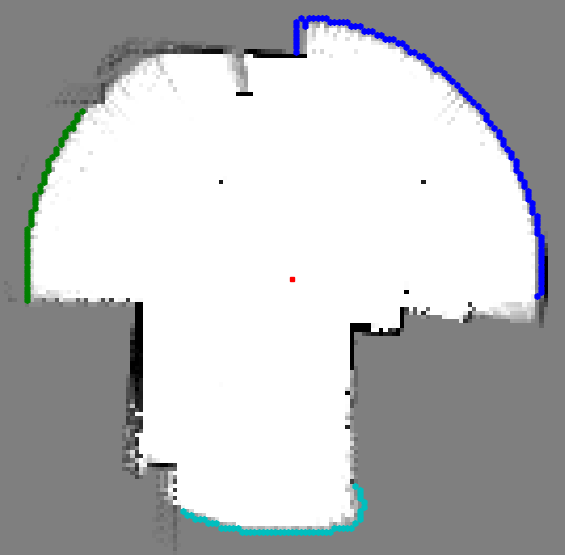
\includegraphics[width=\linewidth]{frontiers_wfd_real_map.png}
        \caption{Frontiers real map WFD}
        \label{fig:frontiers_wfd_real_map}
    \end{subfigure}
\end{figure}

The main difference with our naive approach is of course the efficiency of this last method, it can almost instantaneously find the frontiers in the real map.

\subsection{Choosing the goal point}

Now that we are able to find the frontiers we have to first choose which frontier we want to go to and then what point in this frontier we should choose.
To do so we determined that we should always try to explore the closest frontier, that way the robot will not have to cross through the entire map again and again.

To determine the goal point to go to we decided to choose a point that would be around the middle of the frontier, to do so we have to find the centroid of the selected frontier.

The coordinates of the centroid of a frontier is calculated in that way, with $x_i$ and $y_i$ the points of the frontier:

\begin{align*}
    &x = \dfrac{\sum_{i=0}^{n}x_i}{n}   &y = \dfrac{\sum_{i=0}^{n}y_i}{n}
\end{align*}

The process of finding the frontiers and a goal point is done every 14 seconds or every time the robot reaches the goal point, that way when the frontier moves the robot will follow it.

\section{Reaching the goal}

\subsection{Computation of the force to apply}

Now that we are able to define a goal point we still have to find a way to reach it while avoiding the obstacles.

At first we thought about building a path from the map and then implement an algorithm to avoid the obstacles while tracking the path.
That solution would have worked well but we decided to use a potential field, in that way we have to compute the attractive and repulsive forces to apply to the robot to reach the goal while avoiding the obstacles.

To compute the attractive force we use this method:

\begin{enumerate}
    \item The first step is to compute the length of the vector, we compute the distance in the grid between the robot and the goal and we apply a weight of 0.4 and then limit the maximum length to 18.
    \item Then we compute the angle of the vector, the formula is $atan2(\Delta y, \Delta x)$.
    \item To finish we compute the coordinates of the vector using those formulas: $x: length * cos(angle)$, $y: length * sin(angle)$.
\end{enumerate}

To compute the repulsive force we use the following method:

\begin{enumerate}
    \item We consider a circle area around the robot with a radius of 10.
    \item In this circle we select the 10 closest obstacle, is considered an obstacle a cell with a value greater or equal to 0.75.
    \item Then we compute the 10 corresponding vectors using the same method as for the attractive force. Except that we apply a logarithmic function to the computed length and then apply a weight of 3.5 to each of the computed vectors.
    \item After that we have to add the 10 of them into one vector, to do so we simply sum all the x and y together to obtain the final repulsive vector.
\end{enumerate}

To obtain the general force to apply to the robot we add the x and y of both attractive and repulsive forces together.

In the following figure we can see the forces applied on the robot.
The blue hexagon is the goal point, the green arrow is the attractive force, the red one is the repulsive force and the one in magenta is the general force.
Only half of the points of the frontiers are displayed out to save some time, this is why they are not very clear.

\FloatBarrier
\begin{figure}
    \centering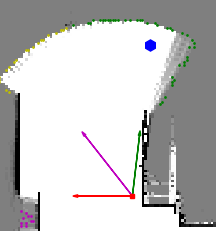
\includegraphics[width=0.5\textwidth]{forces.png}
    \label{fig:forces}
    \caption{Forces applied to the robot}
\end{figure}
\FloatBarrier

\subsection{Convert the force into commands for the robot}

Once the force to apply to the robot computed we have to make the robot orientates itself in the direction of the vector and adapt its speed to the situation.

To do this we created a function in Controller called $apply\_force$, this function uses part of the algorithm we previously developed for the 'follow the path' assignment of the 'Fundamentals of artificial intelligence' course.

The coordinates $x$ and $y$ of the force vector to apply are given in parameters of the function.

\begin{itemize}
    \item[$-$] We first compute the length of the vector using:
        $$\sqrt{x^2 + y^2}$$
    \item[$-$] Then its angle using:
        $$atan2(y, x)$$
    \item[$-$] Then we compute $\Theta$ in that way:
        $$sin(force\_angle - robot\_angle)$$
    \item[$-$] With $\Theta$ we can compute the angular speed, with $max\_ang\_speed$ being $3$ and $weight$ being $0.8$, in that way:
        $$max\_ang\_speed \cdot \Theta \cdot weight$$
    \item[$-$] The angular speed computed is then confined between $-max\_ang\_speed$ and $max\_ang\_speed$.
    \item[$-$] Then we apply the following function to the angular speed to obtain an adapted linear speed:
        $$max(0, 0.5 + log10(-ang\_speed + max\_ang\_speed))$$
\end{itemize}

